\documentclass[a4paper,12pt]{article}
\usepackage[toc,page]{appendix}
\usepackage{listings}
\usepackage{url}
\usepackage{graphicx}
\usepackage[skip=0pt]{caption}
\usepackage{multicol}
\usepackage{float}
\usepackage[margin=1in]{geometry}
%\usepackage{natbib}

\begin{document}

\renewcommand{\thelstlisting}{\thesection.\arabic{lstlisting}}
\renewcommand{\thefigure}{\arabic{section}.\arabic{figure}}
\renewcommand{\thetable}{\arabic{section}.\arabic{table}}
\setlength{\floatsep}{0pt plus 2pt minus 2pt}
%\setlength{\intextsep}{0pt plus 2pt minus 2pt}
%\setlength{\textfloatsep}{0pt plus 2pt minus 2pt}

\title{Introduction to Digital Libraries Assignment \#4}
\date{April 23, 2015}
\author{James Tate II}
\maketitle

\section{Introduction}
Assignment \#4 first required analyzing the changes (if any) in the representations retrieved
in assignment \#3. The same URIs were dereferenced again and compared to the previous
representations. The next part of this assignment involved retrieving TimeMaps of the
analyzed URIs, and analyzing the number of mementos each URI had. The last part of the
assignment required generating graphs of Jaccard Distance over time of 20 URIs.

\section{Methodology}
I wrote two scripts for this utility, both of which are available in my git repository on
GitHub\footnote{\url{https://github.com/jamesbtate/cs851-s15}}.

\subsection{jusText}

\begin{lstlisting}[basicstyle=\ttfamily,caption={Generating list of files in tweets directory}]
    find ./tweets/ > tweets_file_list
\end{lstlisting}

\begin{table}[H]
\centering
\caption{Word Count Data}
\begin{tabular}{ | c | c | c | }
\hline
\textbf{Data Point}  & \textbf{Original} & \textbf{After jusText} \\ \hline
Total bytes          & 646,619,835  & 12,133,748    \\ \hline
Total words          & 33,594,568   & 2,035,935     \\ \hline
Unique words         & 9,135,191    & 121,422       \\ \hline
Total letter words   & 81,318,873   & 2,030,636     \\ \hline
Unique letter words  & 1,271,593    & 57,434        \\ \hline
\end{tabular}
\end{table}

%\begin{figure}[H]
%    \centering
%    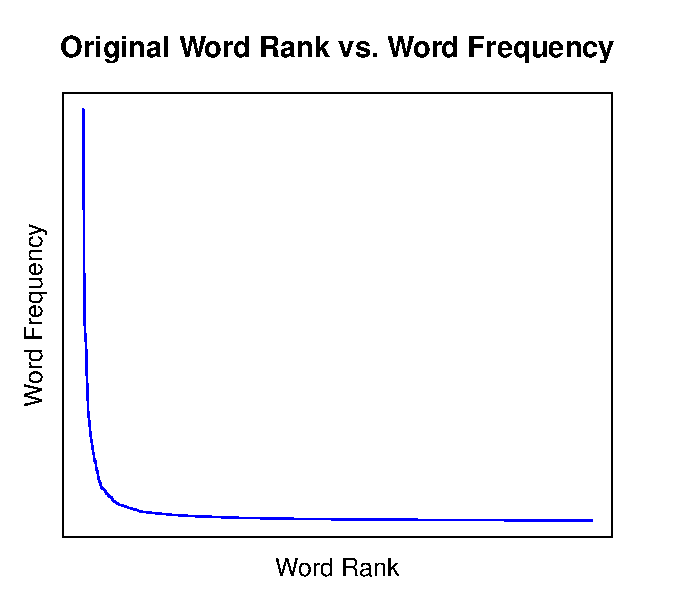
\includegraphics{stats/original_words.pdf}
%    \caption{Rank of Original Words vs. Their Frequency}
%\end{figure}

\bibliographystyle{plain}
\bibliography{../../cs751}

\end{document}
